Nous proposons ici une méthode géométrico-algébrique sans user de la notion de dérivée.
%
Pour ce faire, commençons par symétriser le problème en obtenant une hyperbole symétrique par rapport à la 1\iere\ bissectrice $\setgeo{D}: y = x$.
Il suffit de considérer la fonction $g$ définie sur $\intervalC{0}{\num{3.5}}$ par $g(x) = f(2x) = \frac{7-2x}{2x+2}$. Cette opération algébrique correspond à appliquer une dilatation horizontale de coefficient \num{.5}.

\smallskip

\begin{center}
	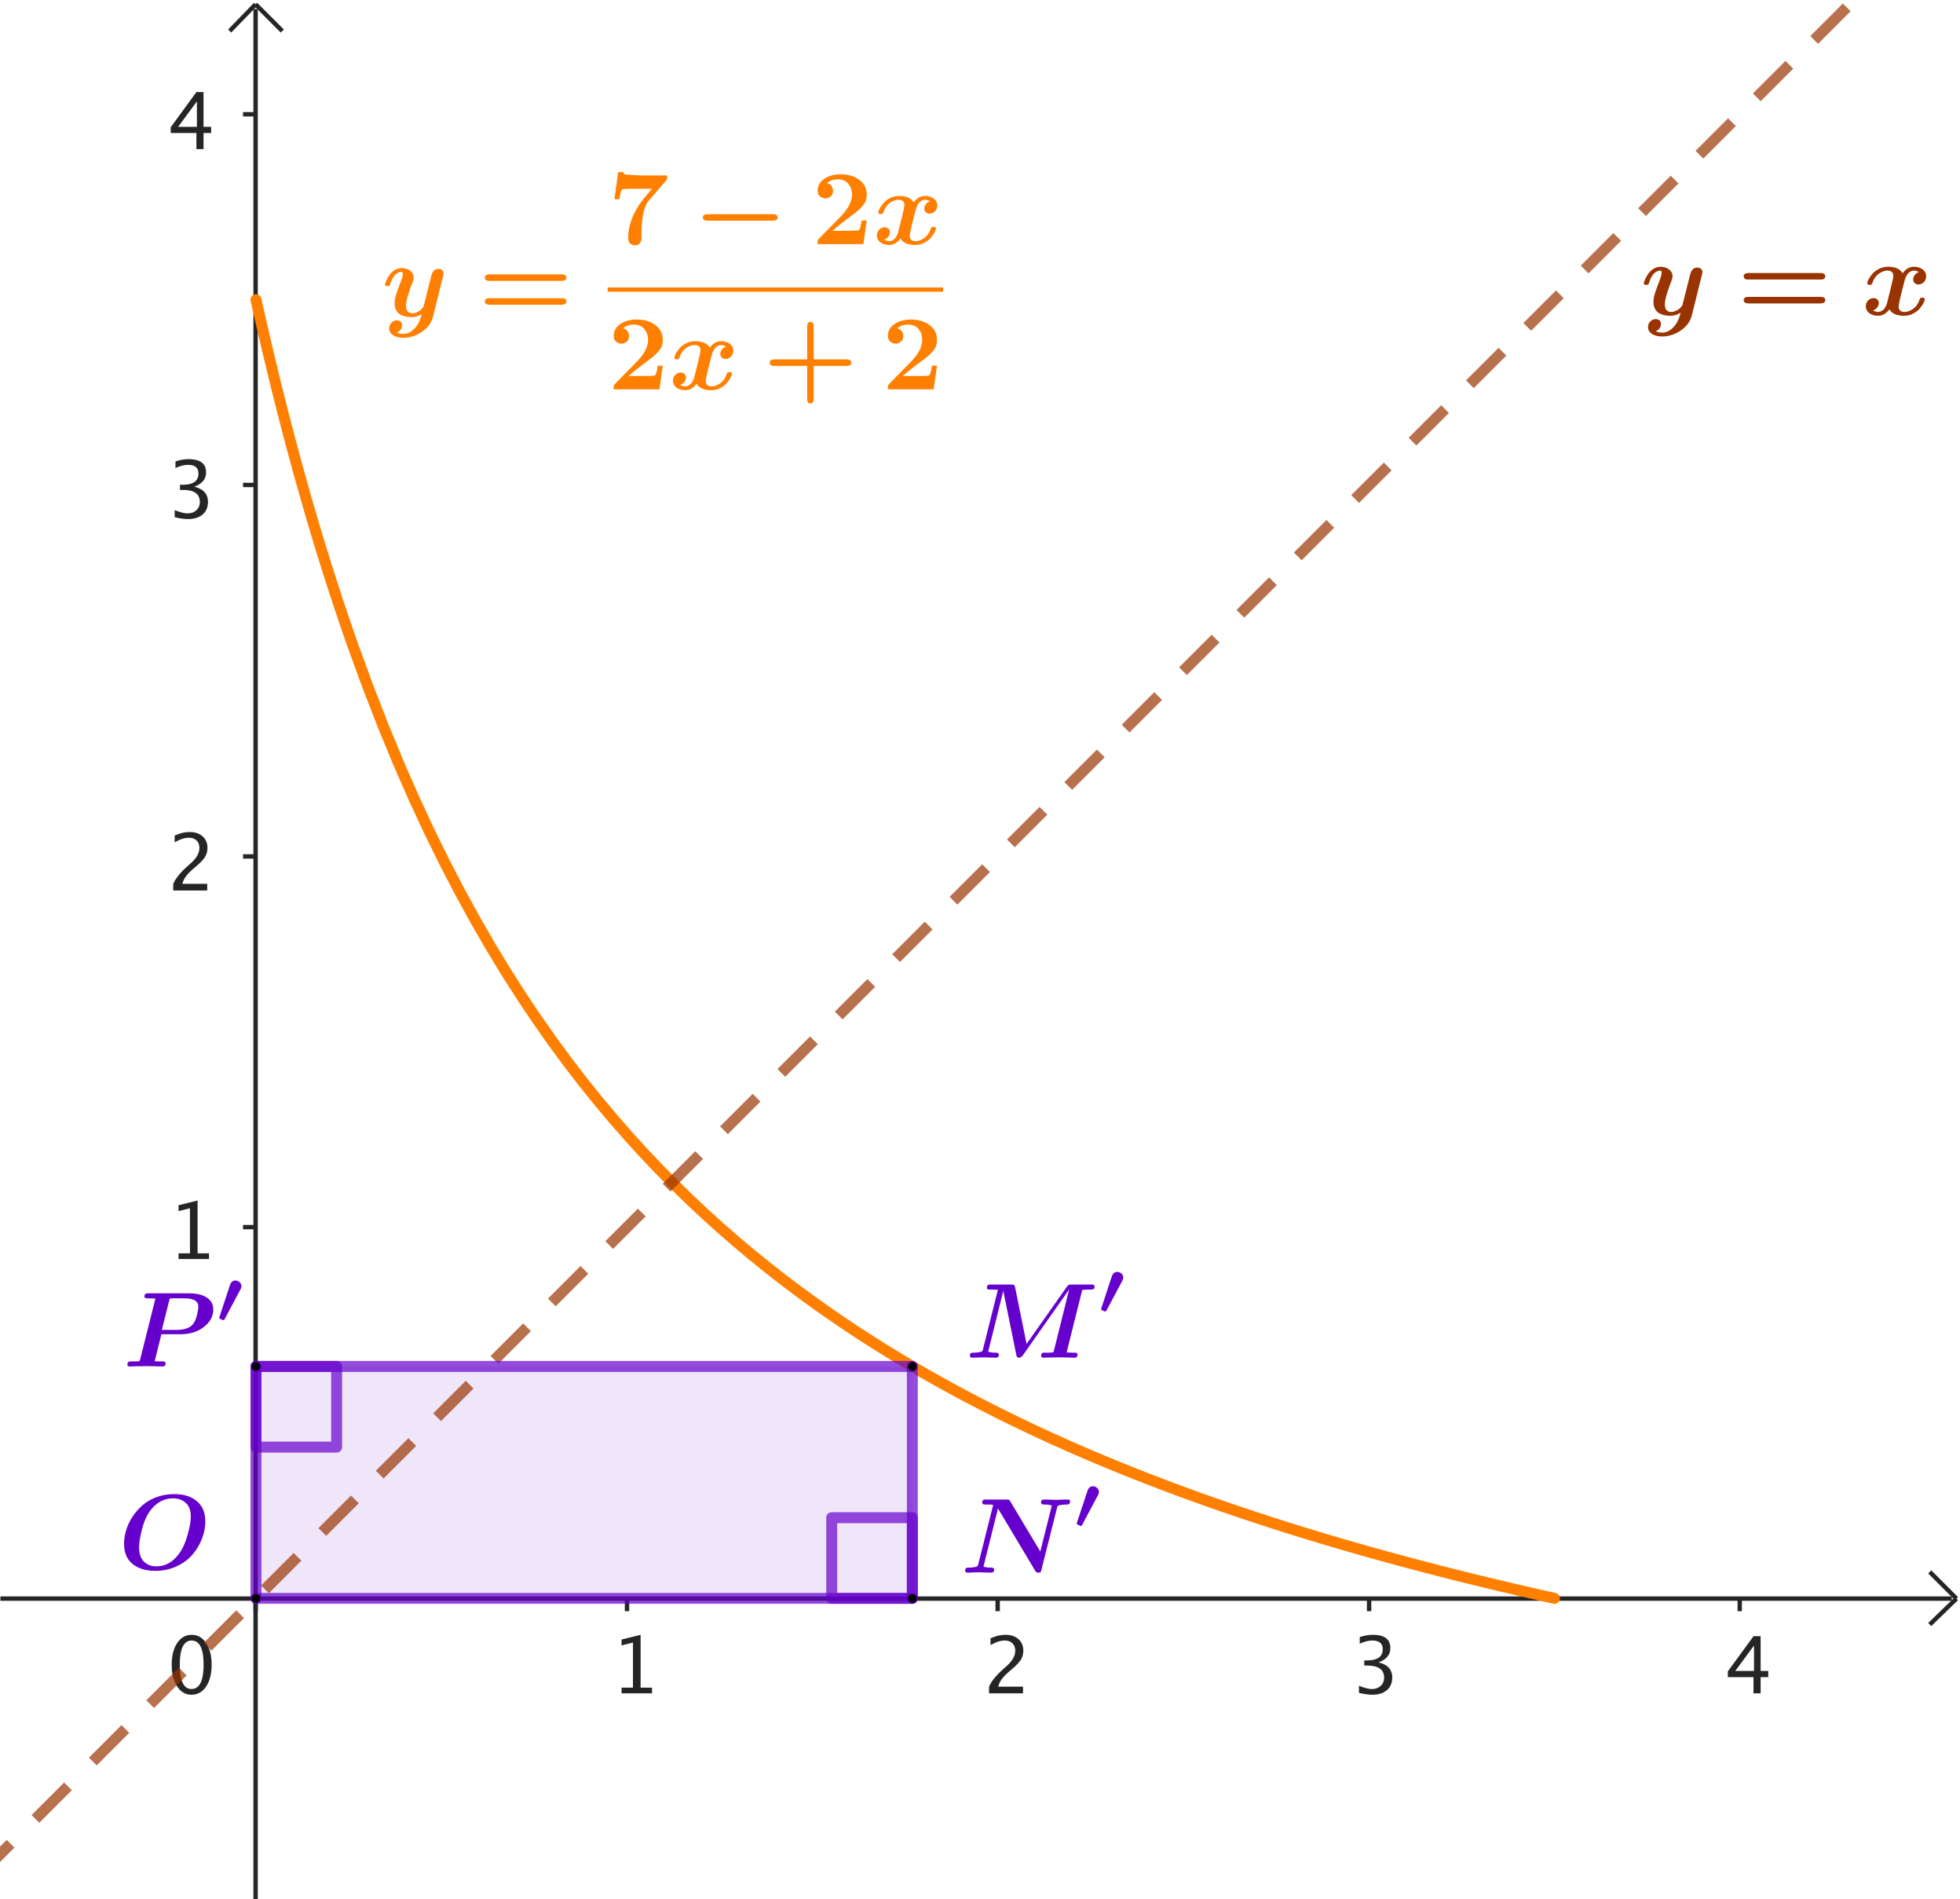
\includegraphics[scale=.67]{symmetric-goal.png}
\end{center}

La calcul suivant démontre que $\setgeo*{C}{g}: y = g(x)$ est bien symétrique rapport à $\setgeo{D}$.

\smallskip
\begin{stepcalc}[style=sar]
	g\big( g(x) \big)
\explnext{}
	     \Big( 7 - 2 \cdot \dfrac{7-2x}{2x+2} \Big)
	\div \Big( 2 \cdot \dfrac{7-2x}{2x+2} + 2 \Big)
\explnext{}
	\dfrac{ 7(2x+2) - 2(7-2x) }{ 2(7-2x) + 2(2x+2) }
\explnext{}
	\dfrac{18 x}{18}
\explnext{}
	x
\end{stepcalc}
\smallskip


% ----------------------- %


Cette propriété de symétrie nous permet de deviner le rôle essentiel de
$\gamma = \num{1.5} \sqrt{2} - 1$, % -1 + 3/sqrt(2)
l'unique solution sur $\intervalC{0}{\num{3.5}}$ de 
$g(x) = x$,
c'est-à-dire de 
$\frac{7-2x}{2x+2} = x$,
soit
$2 x^2 + 4 x - 7 = 0$.
%
Notons alors $\setgeo{A}(x) = x g(x)$ pour $x \in \intervalC{0}{\num{3.5}}$.
Nous allons démontrer, sans dériver, la croissance stricte de $\setgeo{A}$ sur $\intervalC{0}{\gamma}$, et par conséquent sa décroissance stricte sur $\intervalC{\gamma}{\num{3.5}}$ par raison de symétrie.
%
Considérons donc $a$ et $b$ deux réels tels que $0 \leq a < b \leq \gamma$, puis observons le schéma suivant.

\smallskip

\begin{center}
	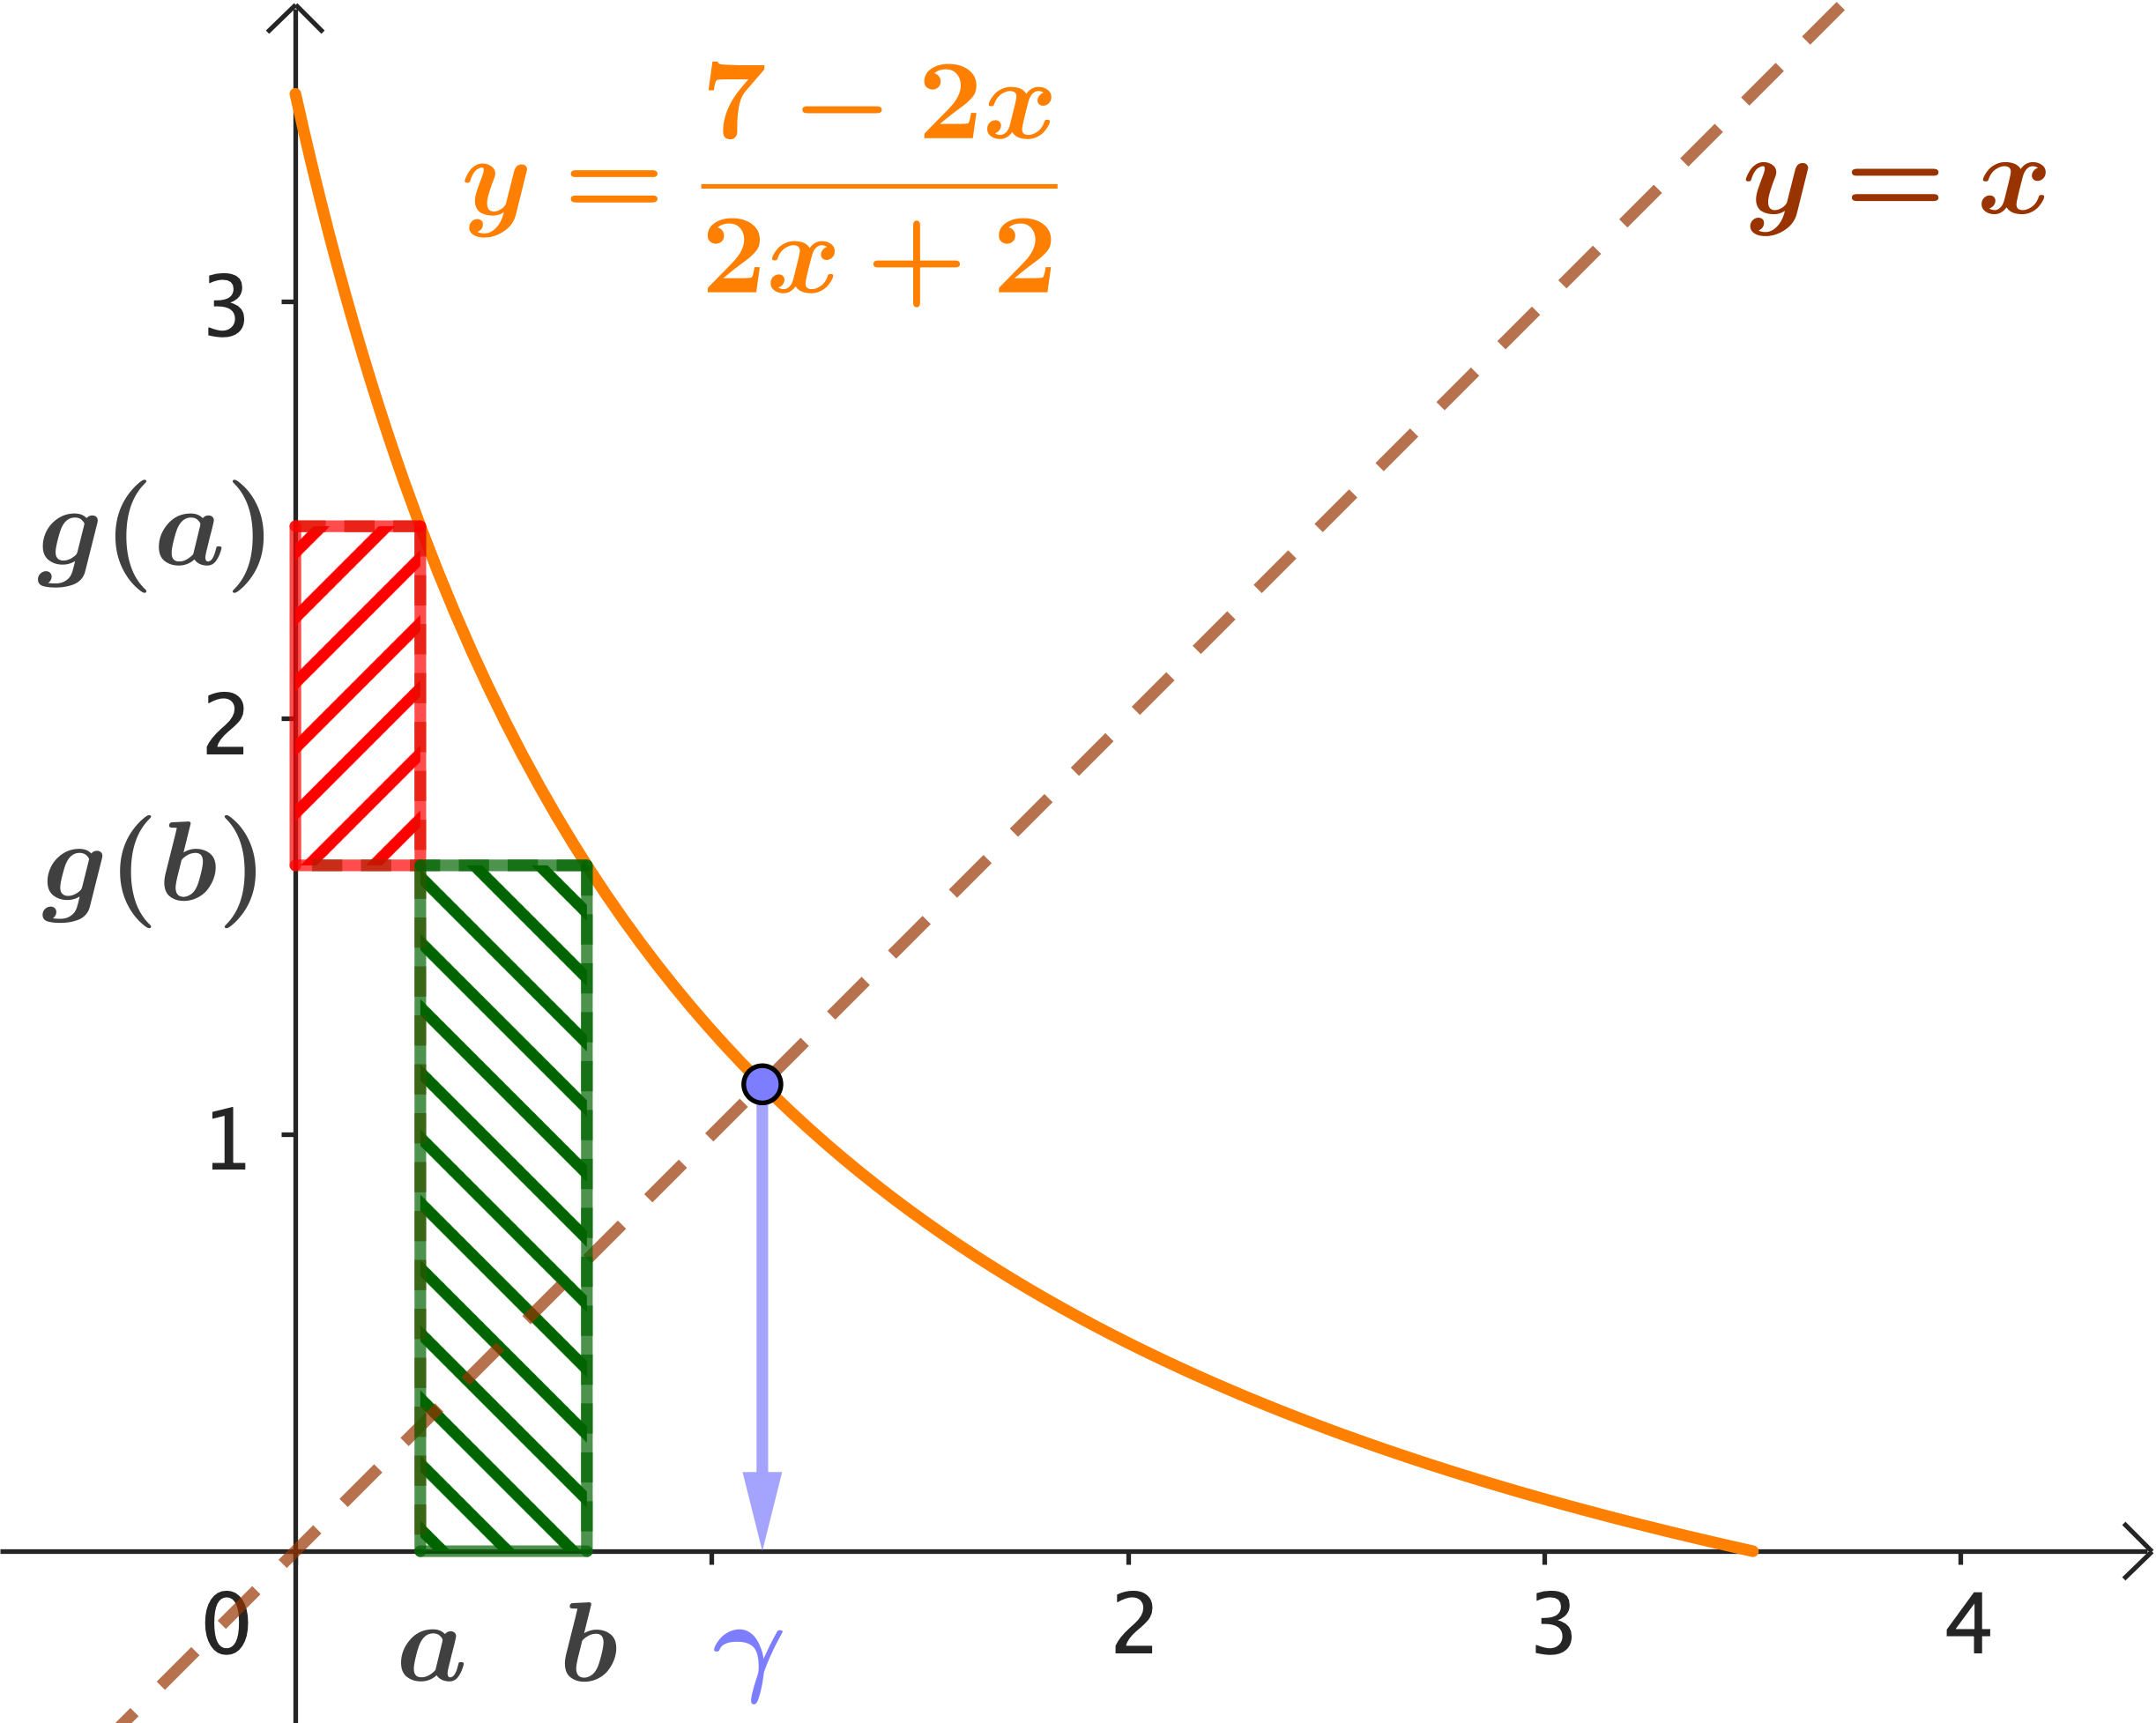
\includegraphics[scale=.67]{geo-sol.png}
\end{center}

Nous avons
$\setgeo{A}(a) < \setgeo{A}(b)$
si, et seulement si,
$a \big( g(a) - g(b) \big) < (b - a) g(b)$.
Nous voilà partis pour un peu de calcul...
%
\begin{itemize}
	\item
	\begin{stepcalc}[style=sar]
		2 \big( g(a) - g(b) \big)
	\explnext{}
		\dfrac{7 - 2a}{a + 1} - \dfrac{7 - 2b}{b + 1}
	\explnext{}
		\dfrac{(7 - 2a)(b + 1) - (7 - 2b)(a + 1)}{(a + 1)(b + 1)} 
%	\explnext{}
%		\dfrac{7b + 7 - 2ab - 2a - 7a - 7 + 2ab + 2b}{(a + 1)(b + 1)}
	\explnext{}
		\dfrac{9(b - a)}{(a + 1)(b + 1)}
	\end{stepcalc}


	\item Le point précédent nous amène aux calculs suivants.

	\smallskip
	\noindent\kern-12pt\begin{stepcalc}[style=ar*]
		\dfrac{2(a+1)(b+1)}{b - a} \big( 
			  a \big( g(a) - g(b) \big) 
			- (b - a) g(b) 
		\big)
%	\explnext{}
%		(a+1)(b+1) \Big( 
%			  \dfrac{2 a \big( g(a) - g(b) \big)}{b - a} 
%			- 2 g(b) 
%		\Big)
	\explnext{}
		  9a - (7 - 2b)(a + 1)
%	\explnext{}
%		9a - 7a - 7 + 2ab + 2b
	\explnext{}
		2a + 2ab + 2b - 7
	\end{stepcalc}


	\item En nous souvenant de $0 \leq a < b \leq \gamma$, nous avons
	$2a + 2ab + 2b - 7 < 2b^2 + 4b - 7$.
	Or, les racines de $2 x^2 + 4 x - 7$ sont $\gamma$ et $\overline{\gamma} = - \num{1.5} \sqrt{2} - 1$, 
	donc $b \in \intervalO{\overline{\gamma}}{\gamma}$ donne 
	$2b^2 + 4b - 7 < 0$, puis 
	$a \big( g(a) - g(b) \big) < (b - a) g(b)$.
\end{itemize}


Nous arrivons au tableau de variations suivant.

\begin{center}
	\begin{tikzpicture}
                \tkzTabInit[espcl=2.5]{
                	$x$              / 1    ,
    				$\setgeo{A}(x)$  / 1.5
    			}{$0$, $\gamma$, \num{3.5}}

                \tkzTabVar{-/ , +/, -/ }
	\end{tikzpicture}
\end{center}

Finalement,
pour revenir à $A(x)$ maximale, il suffit d'inverser la dilatation horizontale qui a permis de passer de $f(x)$ à $g(x)$, soit prendre $2 \gamma = 3 \sqrt{2} - 2$, au lieu de $\gamma$.
%
Finalement,
$\area(MNOP)$ est maximale uniquement lorsque $x_M = 3 \sqrt{2} - 2$.
